\section{Visualiseringssystemet}
Visualiseringssystemet är det delsystem som använder den HDF5-fil som parsersystemet genererar för att visualisera beräkningsresultaten. Detta görs genom olika nätverk, bestående av processorer. Nedstående kapitel redovisar de olika befintliga nätverk ENVISIoN består av. 

\subsection{Nätverk}
För att visualiseringssytemet ska vara kompatibelt med den HDF5-strukturen som parsersystemet genererar kommer utseendet hos nätverken att se olika ut för varje visualisering. Nedan återfinns olika nätverk som olika skript genererar för olika visualiseringar.

\subsubsection{Nätverk för visualisering av parkorrelationsfunktionen}

Ett nytt skript med processorer för visualisering av parkorrelationsfunktionen har utvecklats. Det nätverk som skapas av skriptet visas i figur \ref{fig:PCF}. 
 
\nyBild{PCF.png}{Nätverk för parkorrelationsfunktion.}{PCF}{0.35}

Nätverket startar med att öppna en HDF5-fil. Efter det kontrollerats om gruppen \textit{PairCorrelationFunc} finns i den parsade filen med hjälp av \textit{HDF5PathSelection}-processorn. Därefter läggs det till en \textit{HDF5ToFunction}-processor som extraherar den parsade datan och gör om det till en funktion. Nästkommande processorn, dvs \textit{LinePlot}, används för att
rita upp den data som tas emot från föregående processron. En mesh byggs upp med hjälp av \textit{MeshRenderer}-processorn, \textit{Background}-processorn bygger upp bakgrunden och \textit{TextOverlay}-processorn används för att skriva ut text till canvasen. 
\newpage
Figur \ref{fig:PCF} och \ref{fig:network} demonstrerar ett exempel på ett nätverk och respektive 2D-graf som visualiserar paircorrelation funktionen för Si med 40 steg i temperaturen 300K. Observera att alla \textit{HDF5ToFunction}-processorer inte syns i figur \ref{fig:PCF}. Den 2D-grafen som genereras av nätverken visas i figur \ref{fig:PCF}. 

\nyBild{network.png}{2D-graf från parkorrelationsfunktion.}{network}{0.7}
 




\subsubsection{Bandstruktur}
Nätverket startar med att öppna en HDF5-fil. Därefter kontrolleras om det finns en sökväg med namnet \textit{Fermienergy} i filen, skulle sökvägen existera läggs en processor till som extraherar det värdet sparat i ett dataset. Sedan navigeras det genom HDF5-filen till platsen där alla band är sparade. Alla dessa band sparas i en DataFrame där varje kolumn innehåller alla värden för ett band. Skulle Fermienegin finnas i HDF5-filen kommer det värdet att subtraheras från alla värden i DataFrame. Sedan ritas alla band upp i en graf med samma värden på x-axeln. y-axeln får en rubrik med lämplig text, antigen \textit{Energy} eller \textit{Energy - Fermi energy}, för att sedan visualiseras i ett fönster.

Med den kunskapen gruppmedlemmarna besitter idag skulle inte samma tillvägagångssätt för visualiseringen tagits. Kontrollen av fermienergi skulle ske redan i parsern för bandstrukturen. Skulle Fermienergin hittas, subtraheras värdet redan innan all data för de olika banden lagras i ett dataset.
\nyBild{BandsNetwork.PNG}{Nätverk för visualisering av bandstruktur.}{BandsNetwork}{0.5}
\begin{figure}[ht]
    \begin{subfigure}{.5\textwidth}
        \centering
        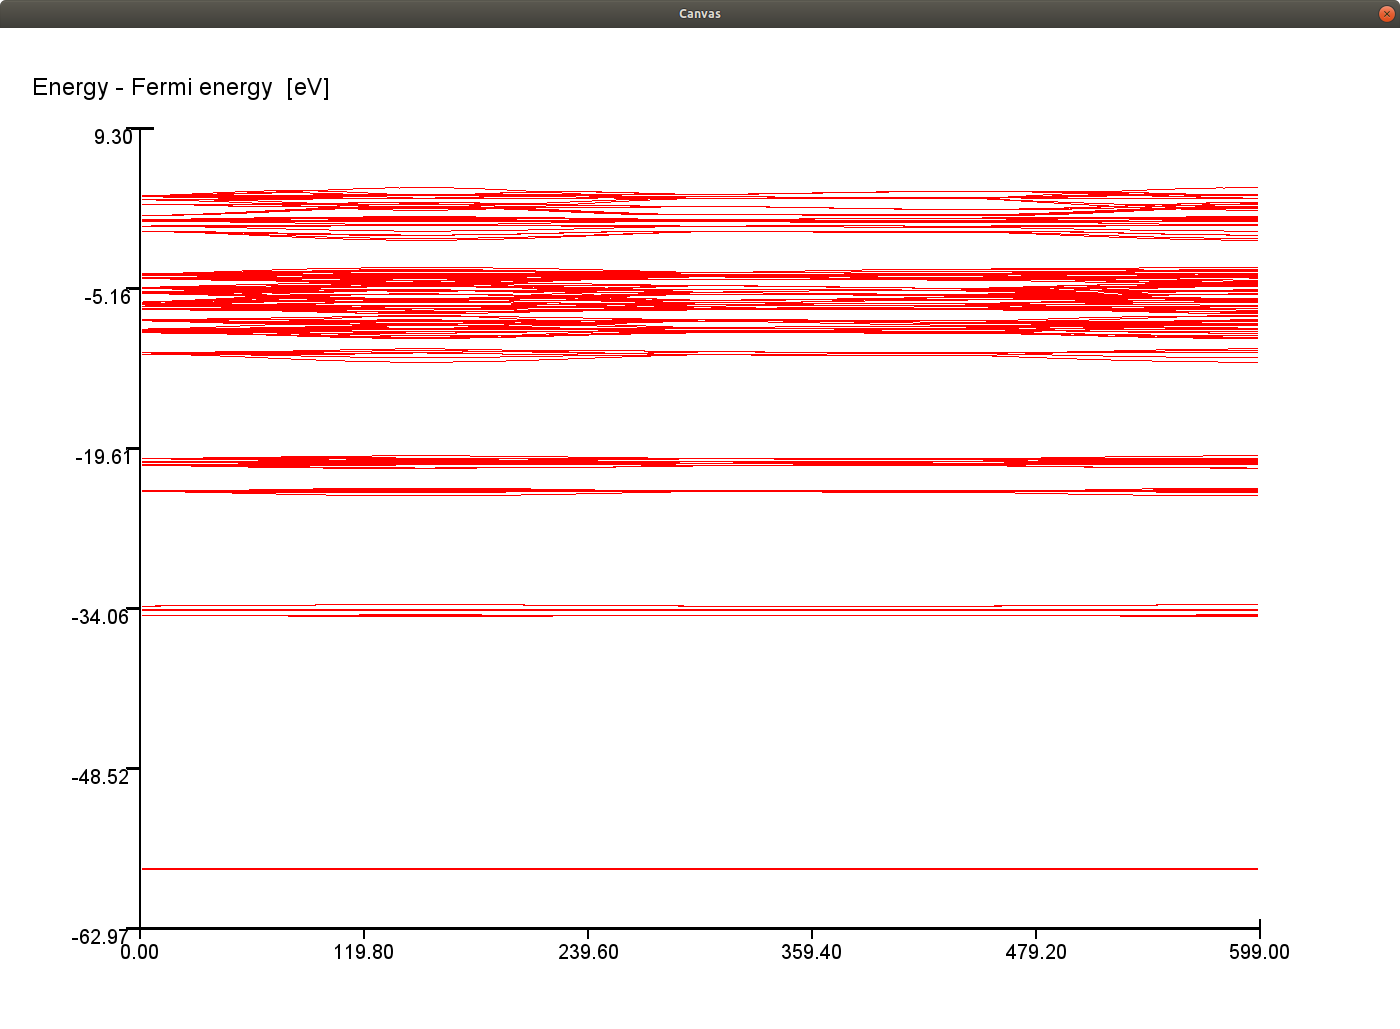
\includegraphics[width=\linewidth]{images/BandsAll.png}
        \caption{Visualisering av hela bandstrukturen som \\skapas när nätverket evalueras.}
        \label{fig:allBands}
    \end{subfigure}%
    \begin{subfigure}{.5\textwidth}
        \centering
        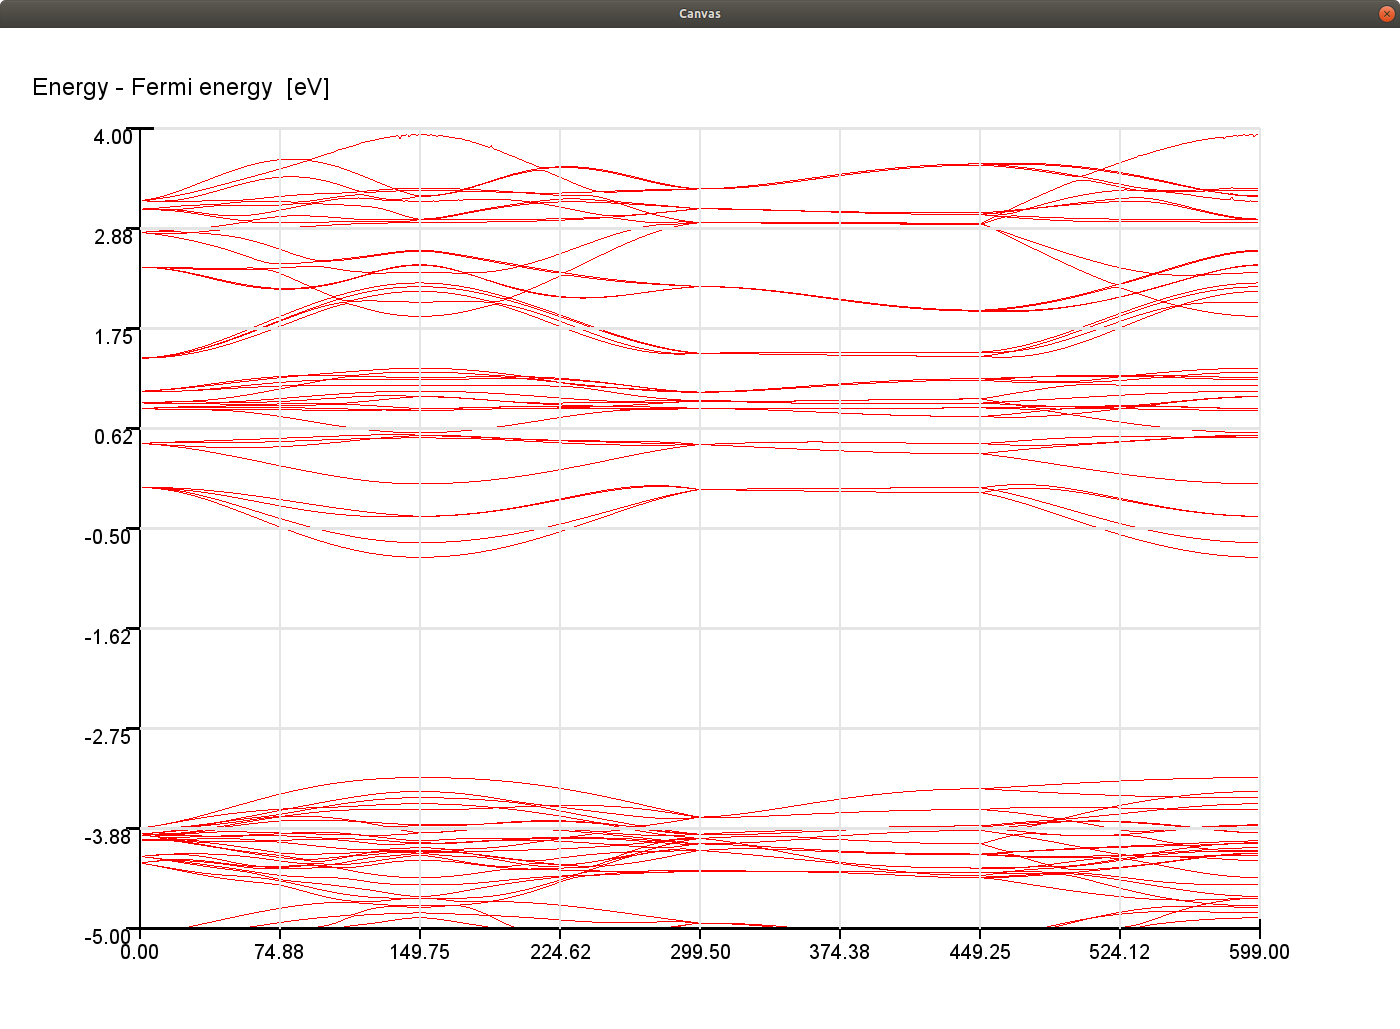
\includegraphics[width=\linewidth]{images/ZoomedBands.png}
        \caption{En förstoring av figur \ref{fig:allBands} där endast energin \\mellan $-4$ eV och $5$ eV visas.}
        \label{fig:zoomedBands}
    \end{subfigure}
    \caption{Visualisering av bandstruktur för TiPO4.}
    \label{fig:Band}
\end{figure}

\subsubsection{Tillståndstäthet}
Nätverket för visualisering av tillståndstäthetsdata laddar en \textit{HDFSource}-processor som anger HDF5-filen som data laddas från. Sedan kopplas en \textit{HDF5PathSelection}-processor, som tar ut den givna HDF5-gruppens alla undergrupper direkt till den redan befintliga \textit{HDFSource}-processorn. Denna processor anger att data ska laddas från DOS-gruppen i HDF5-filen. Två till \textit{HDF5PathSelection}-processorer laddas sedan som anger grupperna Total och Partial i HDF5-filen.  

För Total-delen laddas sedan kontinuerligt \textit{HDF5ToFunction}-processorer som gör funktioner av all 
data i Total-gruppen. För Partial-gruppen laddas en \textit{HDF5PathSelection}-processor som tar ut dataset för en vald atom genom att välja den givna HDF5-filens relevanta undergrupp. Denna processor har namnet \textit{Partial Pick} i nätverket. Därefter laddas \textit{HDF5ToFunction}-processorer för alla dataset i grupperna under Partial-gruppen. 
\newpage
All data matas sedan in i en \textit{LinePlot}-processor som gör en 2D-graf. Detta matas in i en \textit{Canvas}-processor som visar själva grafen. Dessutom finns två textOverlay processorer som skriver ut text för x- och y-axeln. Figur \ref{fig:DoS} visar total tillståndstäthet för titanfosfat, TiPO4. Figur \ref{fig:DoSNetwork} visar nätverket som ger 2D-grafen i figur \ref{fig:DoS}. Användaren kan även välja att visa en 2D-graf av den partiella tillståndstätheten med hjälp av sammma nätverk.
\begin{figure}[ht]
    \centering
    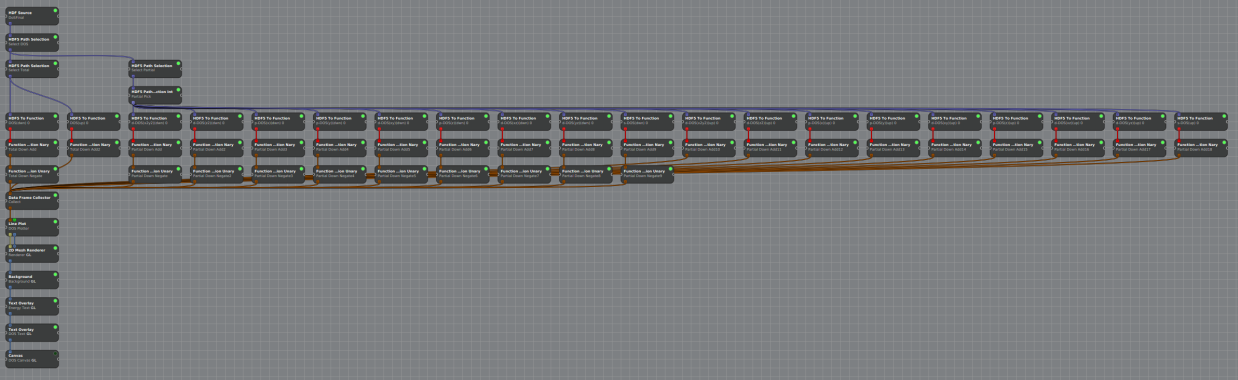
\includegraphics[angle=0, width=\linewidth]{images/DoSNetwork.PNG}
    \caption{Nätverk för visualisering av tillståndstäthet.}
    \label{fig:DoSNetwork}
\end{figure}

\begin{figure}[H]
    \begin{subfigure}{.5\textwidth}
        \centering
        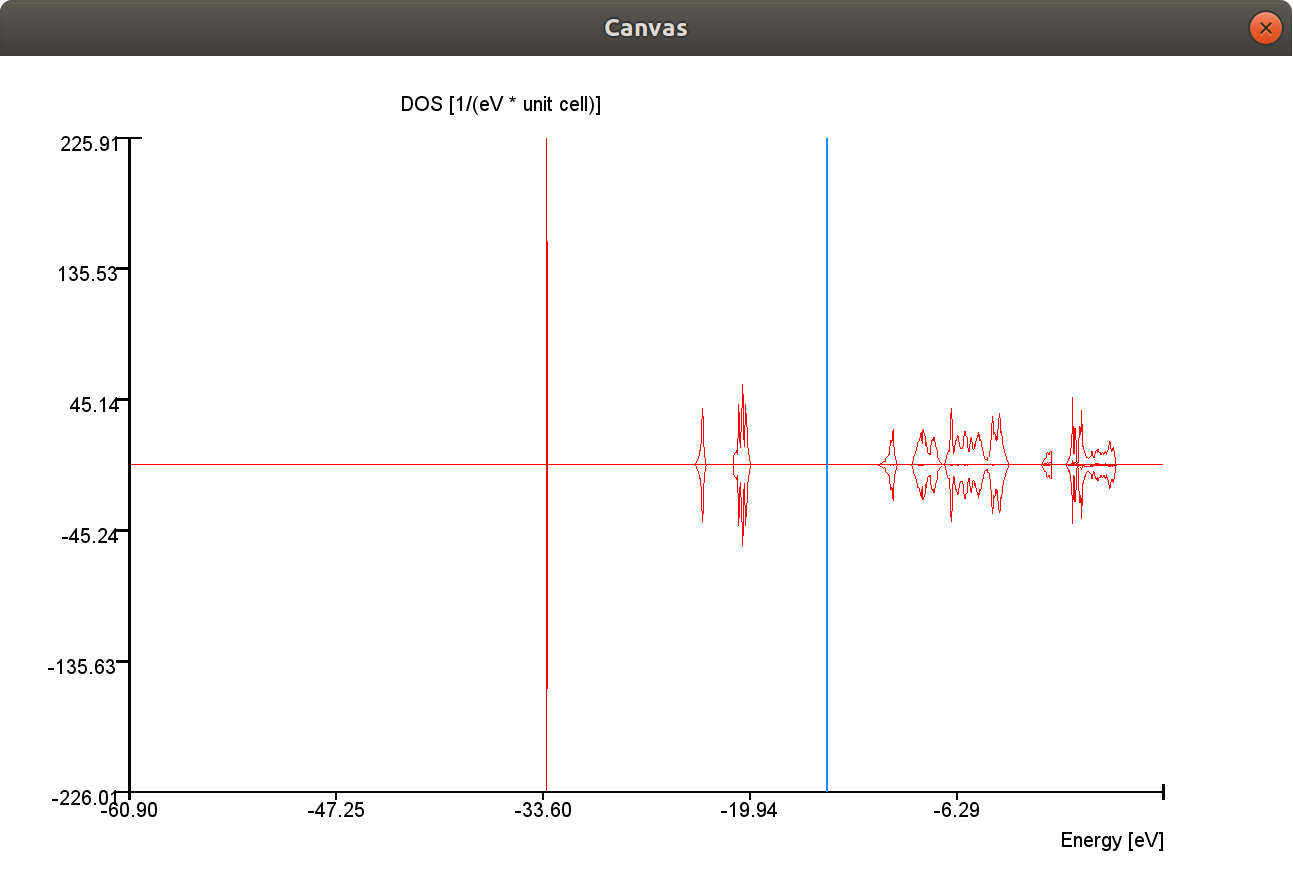
\includegraphics[width=\linewidth]{images/TotalDoS.png}
        \caption{Visualisering av den totala tillståndstätheten \\med en blå hjälplinje för avläsning.}
        \label{fig:totDoS}
    \end{subfigure}%
    \begin{subfigure}{.5\textwidth}
        \centering
        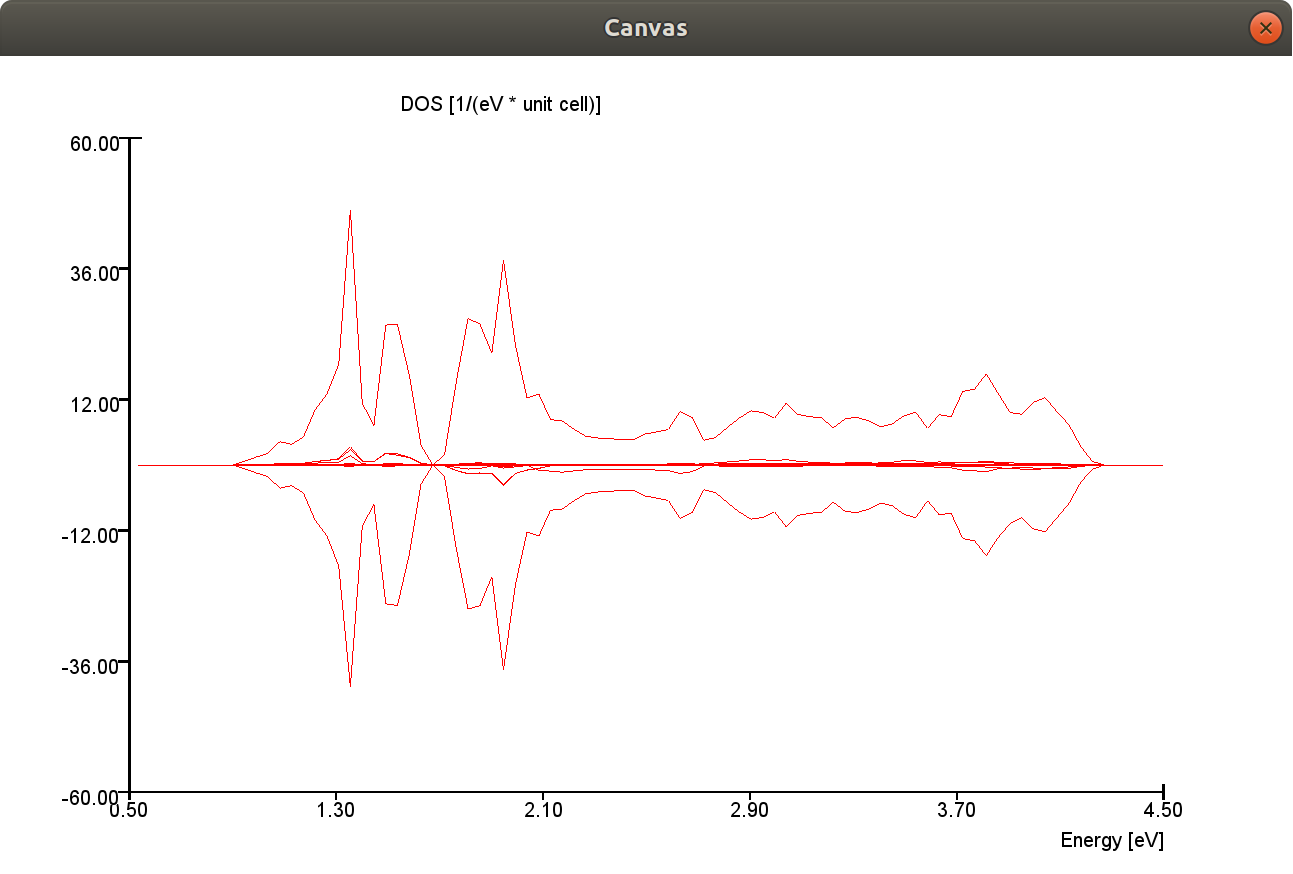
\includegraphics[width=\linewidth]{images/ZoomedDoS.png}
        \caption{Förstoring av visualiseringen av den totala \\tillståndstätheten i figur \ref{fig:totDoS}.}
        \label{fig:zoomedDoS}
    \end{subfigure}
    \caption{Visualisering av tillståndstätheten för TiPO4.}
    \label{fig:DoS}
\end{figure}

\subsection{NetworkHandlers}\label{ssec:NetworkHandlers}
För att andra delsystem enkelt ska kunna sätta upp och ändra parametrar i inviwonätverken så har python-klasser, kallade \textit{NetworkHandlers}, skrivits. Dessa klasser initierar specifika delar av nätverket och har funktioner för att ändra speciella properties i de processorer de har ansvar över. \textit{NetworkHandlers} finns för nuvarande inte för alla visualiseringar utan bara för de relaterade till volymrendering. 

\subsubsection{VolumeNetworkHandler}
En klass som sätter upp ett generiskt nätverk för volymrendering. Nätverket som byggs upp kan inte självstående ge upphåv till någon visualisering då ingen volymdatakälla initieras. Detta måste istället göras från en mer specificerad \textit{VolumeHandler}-klass som ärver denna.

\nyBild{VolumeHandler/volume_network_ex.PNG}{Nätverket som byggs upp då en VolumeNetworkHandler-instans initieras.}{VolumeNetworkHandler}{0.7}

Som visas i figur \ref{fig:VolumeNetworkHandler} så kan nätverket delas upp i två delar. En volymrenderingsdel och en tvärsnittsrenderingsdel.

Processorerna \textit{Cube Proxy Geometry}, \textit{Entry Exit Points}, och \textit{Volume Raycaster}, visade i mitten av figur \ref{fig:VolumeNetworkHandler} kommer att generera bilddata direkt baserat på den volymdata de tar emot.

Processorerna \textit{Volume Bounding Box} och \textit{Mesh Renderer} visade i högra delen av figur \ref{fig:VolumeNetworkHandler} kommer att generera bilddata av den parallellepiped som stänger in volymen. Bilddatan skickas sedan till \textit{Volume Raycaster} och sammanfogas där med bilddatan av volymen. Detta skickas sedan till \textit{Volume Background}-processorn där en bakgrund adderas till bilddatan som sedan skickas till \textit{Canvas}-processorn där den slutgiltiga visualiseringen visas.

Tvärsnittsrenderingen tar emot samma volymdata som volymrenderingen, skickar det till \textit{Volume Slice}-processorn, vilken genererar bilddata baserat på ett plan som skär volymen. Bilddatan skickas sedan till en egen canvas. Volymrenderingens \textit{Raycaster}-processor har förmågan att rita ut ett plan på en godtycklig position i volymen. Detta plan länkas till planet i \textit{Volume Slice}-processorn så att ett delvis transparent plan ritas i volymen på samma position som planet \textit{Volume Slice} använder sig av för att hämta sin data. Tvärsnittsrenderingen kan aktiveras och inaktiveras genom att dess \textit{Canvas}-processor raderas eller läggs till, och att planrenderingen i \textit{Raycaster}-processorn aktiveras eller inaktiveras.
\newpage
Viktiga funktioner i \textit{VolumeNetworkHandler}:
\begin{itemize}
    \setlength\itemsep{0em}
    \item \textbf{setup\_volume\_network: } Bygger upp nätverket som visat i figur \ref{fig:VolumeNetworkHandler}. Notera att volyminportarna ej är anslutna.
    \item \textbf{connect\_volume: } Ansluter alla volym-inportarna till en specificerad volym-outport. Detta måste göras innan en visualisering ska köras, annars har nätverket ingen volymdata att visualisera.
    \item \textbf{show\_volume\_dist: } Ritar upp ett nytt fönster med ett histogram över volymdistributionen i en specificerad HDF5-fil.
    \item \textbf{toggle\_slice\_canvas: } Tar bort eller lägger till \textit{Slice Canvas}-processorn. För att aktivera eller inaktivera tvärsnittsrenderingen.
\end{itemize}

Förutom dessa funktioner har \textit{VolumeNetworkHandler} funktioner för att ändra properties hos de processorer den initierat.

\subsubsection{UnitcellNetworkHandler}
En klass som sätter upp ett och hanterar nätverk för atompositionsrendering. Nätverket som sätts upp kan självstående generera en visualisering för bara atompotitioner men kan också kombineras med andra nätverk genom att denna ärvs i mer specificerade \textit{NetworkHandler}-klasser.

\nyBild{VolumeHandler/unitcell_network.PNG}{Nätverket som byggs upp då en UnitcellNetworkHandler-instans initieras.}{unitcell_network}{0.5}

\nyBild{VolumeHandler/unitcell_vis.PNG}{Resulterande bild från nätverk i figur\ref{fig:unitcell_network}}{unitcell_vis}{0.5}

\textit{UnitcellNetworkHandler} börjar med kontrollera att den givna HDF5-filen har data för en atompositionsvisualisering och kastar ett \textit{AssertionError} om den inte har det. Den fortsätter sedan med att sätta upp en \textit{HDF5 Source}-processor, om en sådan redan existerar så används den existerande processorn istället. Vilka atomtyper som HDF5-filen innehåller information om läses sedan. 

En \textit{Coordinate Reader}-processor för varje atomtyp  läggs till. Koordinatdatan skickas vidare till en \textit{Structure Mesh}-processor, en ENVISIoN processor som konverterar koordinaterna till en \textit{mesh}. Meshen skickas till \textit{Sphere Renderer} där den konverteras till bilddata med en sfär vid varje tidigare koordinat. Bilddatan ritas sedan ut på en \textit{Canvas}.

Viktiga funktioner i \textit{UnitcellNetworkHandler}:
\begin{itemize}
    \setlength\itemsep{0em}
    \item \textbf{setup\_unitcell\_network: } Bygger upp nätverket som visat i figur \ref{fig:unitcell_network}.
\end{itemize}

Förutom dessa funktioner har \textit{UnitcellNetworkHandler} funktioner för att ändra properties hos de processorer den initierat.


\subsubsection{ChargeNetworkHandler}
En specificerad klass för att sätta upp och hantera laddningstäthetsvisualiseringen. Klassen genererar ett fullständigt nätverk för laddningstäthetsvisualisering och har funktioner för att alla parameterändringar som där behövs. Ärver \textit{UnitcellNetworkHandler} och \textit{VolumeNetworkHandler} för att hantera atompositions- respektive volymrenderingsaspekten av visualiseringen.  

\nyBild{VolumeHandler/charge_network_ex.PNG}{Nätverket som byggs upp då en ChargeNetworkHandler-instans initieras och HDF5-filen innehåller unitcell-data.}{charge_network}{0.4}

\nyBild{VolumeHandler/charge_vis.PNG}{Resulterande bild från nätverk i figur \ref{fig:charge_network}.}{charge_vis}{0.5}

\textit{ChargeNetworkHandler} börjar med kontrollera att den givna HDF5-filen har data för en laddningstäthetsvisualisering och kastar ett \textit{AssertionError} om den inte har det. Den fortsätter sedan med att initera sina superklasser \textit{VolumeNetworkHandler} och \textit{UnitcellNetworkHandler}. Dessa sätter up sina delar av nätverket som indikerat i figur \ref{fig:charge_network}. 

En \textit{HDF5 Source} sätts upp, denna ansluts till unitcell-delen av nätverket. En \textit{HDF5 To Volume} sätts upp och anslutes till \textit{HDF5 Source}. \textit{HDF5 To Volume} hämtar ut volymdata från HDF5-filens \textit{/CHG/} sökväg. Processorn genererar volymdata som i 
sin tur ansluts med volymrenderingsdelens volymdatainportar. 

\newpage

Bilddatautporten från \textit{Sphere Renderer} ansluts till \textit{Mesh Renderer}. Detta gör att bilderna från de två processorerna slås samman och att både atompoisitoner och volymdata renderas i samma fönster. Även \textit{Sphere Renderer}-processorns \textit{Camera}-property ansluts till \textit{Mesh Renderer} för att kameravinklarna ska vara identiska.

\textit{ChargeNetworkHandler} inaktiverar som standard \textit{Slice Canvas}:en och \textit{Unitcell Canvas}:en. Dessa kan återaktiveras via sina respektive funktioner igen, exempelvis då en knapp i det grafiska gränssnittet klickas på.

Om HDF5-filen inte innehåller unitcell-data så kan \textit{UnitcellNetworkHandler} inte initieras och kastar ett exception. Endast volymrenderingsdelen av visualiseringen initieras då och atompositionsvisualiseringen ignoreras. 

Viktiga funktioner i \textit{ChargeNetworkHandler}:
\begin{itemize}
    \setlength\itemsep{0em}
    \item \textbf{setup\_charge\_network: } Bygger upp nätverket som visat i figur \ref{fig:charge_network}.
    \item \textbf{get\_available\_bands: } Returnerar en lista med de möjliga bandvalen som är möjliga i HDF5-filen.
\end{itemize}

Förutom dessa funktioner har \textit{ChargeNetworkHandler} funktioner för att ändra properties hos de processorer den initierat.

\subsubsection{ELFNetworkHandler}
ELFNetworkHandler är identisk i jämförelse med ChargeNetworkHandler med ett fåtal skillnader. Volymdata från HDF5-filen hämtas från sökvägen \textit{/ELF/} istället för \textit{/CHG/}. Detta gör att funktioner för att hämta och sätta aktiva band också är olika. 

\subsubsection{ParchgNetworkHandler}
En specificerad klass för att sätta upp och hantera visualiseringen för partiell laddningstäthet. Ärver \textit{VolumeNetworkHandler} och \textit{UnitcellNetworkHandler} för att hantera volymrenderingsaspekten respektive atompositionsaspekten av visualiseringen.


\nyBild{VolumeHandler/parchg_network_ex.png}{Nätverket som byggs av ParchgNetworkHandler (utan atompositionsrendering).}{parchg_network}{0.6}

Till att börja med initieras superklassen \textit{VolumeNetworkHandler} detta sätter upp det generiska volymrenderingsnätverket. 

Efter detta initieras volymdatakällan och volymdataoutporten ansluts till volymrenderingsdelen av nätverket. 

Volymkällan är här mer komplicerad i jämförelse mot övriga visualiseringar, eftersom flera olika volymdataset här ska visualiseras som en volym. Precis hur denna del ser ut beror på de bandval som görs av användaren.

\nyBild{VolumeHandler/parchg_source_ex.png}{Exempel på nätverkets volymdatakälla med ett bandval för varje läge.}{parchg_source}{0.5}

Den partiella laddningstäthetsvisualiseringen tillåter användaren att välja ett godtyckligt antal band som ska visualiseras och ett av fyra olika lägen för varje band. Dessa lägen är \textit{Total}, \textit{Magnetic}, \textit{Up-spin}, och \textit{Down-spin}. De olika lägena hämtar ut volymdata ur HDF5-filen på olika sätt.

\begin{itemize}
    \setlength\itemsep{0em}
    \item \textbf{Total: } Hämtar direkt volymdatan från det valda bandets \textit{/total/} sökväg.
    \item \textbf{Magnetic: } Hämtar direkt volymdatan från det valda bandets \textit{/magnetic/} sökväg.
    \item \textbf{Up-spin: } Hämtar ut både \textit{/total/} och \textit{/magnetic/} volymdatan som \textit{v1} och \textit{v2}. Volymerna summeras sedan med formeln \textit{0.5*(v1+v2)}
    \item \textbf{Down-spin: } Hämtar ut både \textit{/total/} och \textit{/magnetic/} volymdatan som \textit{v1} och \textit{v2}. Volymerna summeras sedan med formeln \textit{0.5*(v1-v2)}
\end{itemize}

Volymdatan från de olika bandvalen kombineras sedan med en \textit{Volume Merger}-processor. \textit{Volume Merger} kan summerar upp till fyra volymer till en. Om mer än fyra bandval har gjorts så används flera lager av \textit{Volume Merger}-processorer för att kunna summera alla dessa till en. Volymdatan från den sista \textit{Volume Merger} skickas sedan till volymrenderingsnätverket.

Viktiga funktioner i \textit{ParchgNetworkHandler}:
\begin{itemize}
    \setlength\itemsep{0em}
    \item \textbf{setup\_hdf5\_source: } Initierar \textit{HDF Source}-processorn
    \item \textbf{setup\_band\_processors: } Sätter upp nätverket som hämtar ut och kombinerar volymdata baserat på bandval och lägen. Funktionen kan kallas flera gånger efter att nätverket har startats för att byta bandval och lägen.
\end{itemize}

\newpage

\subsubsection{Plannerade NetworkHandlers}
NetworkHandler-klasser har inte skrivits för alla visualiseringar, de gamla visualiseringsskripten används fortfarande för att starta de tvådimensionella visualiseringarna. För att underlätta underhåll av systemet så bör dessa färdigställas i framtiden. I nuläget finns funktionaliteten för att starta och styra dessa visualiseringar utspridd mellan flera olika filer på olika platser. 
\begin{itemize}
    \setlength\itemsep{0em}
    \item \textbf{LinePlotNetworkHandler: } Skulle hantera den generella delen av en 2D-graf visualisering. Styr allt som har med 2D-grafen att göras, som skalning, axlar på grafen, med mera.
    \item \textbf{BandstructureNetworkHandler: } Ärver LinePlotNetworkHandler och sätter upp den specifika delen för bandstructure visualiseringen. Skulle styra HDF5-källan och  bandval.
    \item \textbf{DOSNetworkHandler: } Ärver LinePlotNetworkHandler och UnitcellNetworkHandler och sätter upp den specifika delen för tillståndstäthets visualiseringen. Skulle styra HDF5-källan och val av tillstånd.
    \item \textbf{PCFNetworkHandler: } Ärver LinePlotNetworkHandler och sätter upp den specifika delen för parkorrelationsfunktions visualiseringen.Skulle styra HDF5-källan och val av tidssteg.
\end{itemize}

\newpage
\subsection{Datastrukturer}
\label{ssec:datastrukturer}
Två datastrukturer, Point och Function, har introducerats. En datastruktur är en form av behållare av olika typer av data som kan skickas mellan processorer. Dessa används i vissa av de implementerade processorerna.
\subsubsection{Point}
Denna datatyp representerar en reell 1D-punkt och inkapslar punktens värde (ett flyttal) samt variabel metadata.
\subsubsection{Function}
Denna datatyp representerar en reellvärd funktion av en reell variabel och inkapslar sampelvärden och variabel-metadata för x- och y-axlarna.

\subsection{Processorer}
\label{ssec:processorer}
För att kunna omvandla den data som översatts från VASP-beräkningar till en visualisering krävs processorer som utför specifika uppgifter. Figur 2 demonstrerar ett typiskt utseende på en processor.
\nyBild{processor.png}{Exempel på en processors utseende.}{processor}{0.8}
De färgade rutorna till vänster på processorn i figur \ref{fig:processor} är olika typer av ingångar och utgångar. Cirkeln i det övre högra hörnet på processorn i samma figur är en lampa som lyser då processorn är aktiv. De processorer som ENVISIoN skapat kategoriseras och beskrivs nedan.

\subsubsection{Kristallstruktur}
\label{ch:kristallstruktur-processorer}
Nedanstående processorer är relaterade till visualiseringen av kristallstrukturer. De tillhör en modul vid namn Crystalvisualization.

\textbf{\textit{CoordinateReader}} \newline
Från en HDF5-fil läser denna processor koordinater för atompositioner. En sökväg till ett dataset sätts via en StringProperty. Utdata från CoordinateReader är $n$ stycken vec3.

Inport:
\begin{itemize}
\item Hdf5::Inport inport\_
\end{itemize}

Utport:
\begin{itemize}
\item DataOutport< std::vector<vec3> > outport\_
\end{itemize}

Properties:
\begin{itemize}
\item StringProperty path\_
\end{itemize}

\textbf{\textit{StructureMesh}} \newline
Atompostionsdata kopplas ihop med rätt atomfärg och radie med StructureMesh-processorn. StructureMesh har en multiinport, dit en eller flera CoordinateReader-processorer kan kopplas in. Indata för StructureMesh är atompositionsdata i form av vec3 för varje atomslag. Till denna indata läggs properties för färg, radie och antal till för varje atomslag/processor som kopplas in. Den ger en mesh, som har buffrar för position, färg och radie.

Inport:
\begin{itemize}
\item DataInport< std::vector<vec3>, 0> structure\_
\end{itemize}

Utport:
\begin{itemize}
\item MeshOutport mesh\_
\end{itemize}

Properties:
\begin{itemize}
    \setlength\itemsep{0em}
    \item FloatProperty scalingFactor\_
    \item FloatMat3Property basis\_
    \item BoolProperty fullMesh\_
    \item IntProperty timestep\_
    \item std::vector< std::unique\_ptr<FloatVec4Property> > colors\_: vektor som innehåller färgproperty för varje atomslag
    \item std::vector< std::unique\_ptr<FloatProperty > > radii\_: vektor som innehåller radieproperty för varje atomslag
    \item std::vector< std::unique\_ptr<IntProperty> > num\_: vektor som innehåller antalet atomer per tidssteg för varje atomslag
    \item BoolProperty enablePicking\_: sann då picking-funktionen är påslagen 
    \item IntVectorProperty inds\_: vektor med index på valda atomer
\end{itemize}

\subsubsection{HDF5}
\label{ch:hdf5-processorer}
Nedanstående processorer är ämnade att fungera väl med de HDF5-relaterade processorer som är inkluderade i Inviwo.

\textbf{\textit{HDF5PathSelection*}} \newline
Detta är en grupp av processorer som har funktionalitet liknande den inbyggda processorn HDF5PathSelection. En eller flera av dessa processorer placeras med fördel mellan en HDFSource och en eller flera HDF5To*.

Gemensamt för dessa processorer är  att de på inporten tar en Hdf5-grupp och på utporten skriver noll eller flera av dessa omedelbara undergrupper.

Nedan beskrivs de olika processorerna i denna grupp.

\textbf{HDFpathSelectionInt} \newline
Denna processor väljer en HDF5-grupp med heltalsnamn, baserat på värdet på processorns intProperty\_, eventuellt utökat med ledande nollor till bredden specificerat på processorns zeroPadWidthProperty\_.

HDF5PathSelectionInt kan med fördel användas tillsammans med en OrdinalPropertyAnimator för att plocka ut relevant data ur en HDF5-fil.

Anledningen till att utdata ges som en vektor av HDF5-grupper, trots att processorn alltid skriver exakt en grupp på utporten, är att processorn ska följa samma mönster som, och fungera väl med, resterande processorer.

Inport:
\begin{itemize}
\item DataInport<hdf5::Handle> hdf5HandleInport\_
\end{itemize}

Utport:
\begin{itemize}
\item DataOutport< std::vector<hdf5::Handle> > hdf5HandleVectorOutport\_
\end{itemize}

Properties:
\begin{itemize}
    \setlength\itemsep{0em}
    \item IntProperty intProperty\_
    \item IntSizeTProperty zeroPadWidthProperty\_
\end{itemize}

\textbf{HDF5PathSelectionIntVector} \newline
Denna processor väljer noll eller flera HDF5-grupper med heltalsnamn, baserat på värdet på processorns intVectorProperty\_, eventuellt utökat med ledande nollor till berdden specificerat av processorns zeroPadWidthProperty\_. 

HDF5PathSelectionIntVector kan med fördel användas tillsammans med ''picking'' för att plocka ut relevant data ur en HDF5-fil.

Inport:
\begin{itemize}
\item DataInport<hdf5::Handle> hdf5HandleInport\_
\end{itemize}

Utport:
\begin{itemize}
\item DataOutport< std::vector<hdf5::Handle> > hdf5HandleVectorOutport\_
\end{itemize}

Properties:
\begin{itemize}
    \setlength\itemsep{0em}
    \item IntVectorProperty intVectorProperty\_
    \item IntSizeTProperty zeroPadWidthProperty\_
\end{itemize}

\textbf{HDF5PathSelectionAllChildren}\newline
Denna processor väljer den givna HDF5-gruppens alla undergrupper.

Inport:
\begin{itemize}
\item DataInport<hdf5::Handle> hdf5HandleInport\_
\end{itemize}

\textbf{\textit{HDF5To*}}\newline
Detta är en grupp av processorer som har funktionalitet liknande den inbyggda processorn HDF5ToVolume. Processorerna placeras med fördel efter en HDFSource-processor, med en eller flera mellan liggande HDF5PathSelection*.

Gemensamt för dessa är att de som indata tar noll eller flera HDF5-grupper (baserat på *pathSelectionProperty\_), plockar ut dataset för varje grupp och omvandlar dessa till relevanta objekt (Point eller Function) som sedan skrivs till utporten. Objektens variabel-metadata tas, om de finns tillgängliga, från attributen associerade med dataseten. Vidare kan, om så väljs med *namePrependParentsProperty\_, metadat utökas med namnen på de grupper var i dataseten ligger.

Vilka dataset som kan väljas med *pathSelectionProperty\_ uppdateras dynamiskt beroende på vilka grupper som ligger på inporten. När ett lämpligt dataset valts kan *pathFreezeProperty\_ användas för att stänga av denna dynamik, så att värdet sparas även om grupperna på inporten (antagligen tillfälligt) ändras. Detta underlättar manuellt experimenterande samt användandet av processorer som tillfälligt ger noll grupper som utadat, t.ex. HDF5PathSelectionIntVector.

\textbf{HDF5ToPoint} \newline
Denna processor konverterar HDF5-data till noll eller flera Point-objekt.

Inport:
\begin{itemize}
\item DataInport<hdf5::Handle, 0, true> hdf5HandleFlatMultiInport\_
\end{itemize}

Utport:
\begin{itemize}
\item DataOutport< std::vector<Point> > pointVectorOutport\_
\end{itemize}

Properties:
\begin{itemize}
    \setlength\itemsep{0em}
    \item OptionPropertyString pathSelectionProperty\_
    \item BoolProperty pathFreezeProperty\_
    \item IntSizeTProperty namePrependParentsProperty
\end{itemize}

\textbf{HDF5ToFunction}\newline
Denna processor konverterar HDF5-data till noll eller flera Function-objekt. 

Normalt plockas två dataset per grupp ut, ett för x-axeln och ett för y-axeln. Om endast data för y-axeln finns tillgänglig kan implicitXProperty\_ sättas, varvid processorn automatgenererar data för x-axeln.

Inport:
\begin{itemize}
\item DataInport<hdf5::Handle, 0, true> hdf5HandleFlatMultiInport\_
\end{itemize}

\newpage

Utport:
\begin{itemize}
\item DataOutport< std::vector<Function> > functionVectorOutport\_
\end{itemize}

Properties:
    \begin{itemize}
    \setlength\itemsep{0em}
    \item BoolProperty implicitXProperty\_
    \item OptionPropertyString xPathSelectionProperty\_
    \item OptionPropertyString yPathSelectionProperty\_
    \item BoolProperty xPathFreezeProperty\_
    \item BoolProperty yPathFreezeProperty\_
    \item IntSizeTProperty xNamePrependParentsProperty\_
    \item IntSizeTProperty yNamePrependParentsProperty\_
\end{itemize}

\subsubsection{2D}
\label{ch:2d-processorer}
Nedanstående processorer är ämnade att bearbeta och presentera 2D-data, närmare bestämt data av typen Point och Function.

\textbf{\textit{FunctionOperationUnary}}\newline
Denna processor implementerar en unär operator, antingen negation $(g_{i}(x) = -f_{i}(x))$ eller (multiplikativ) inversion $(g_{i}(x) = 1/f_{i}(x))$. Operatorn appliceras på funktioner på inporten, en i taget, och skriver respektive resultat på utporten.

Inport:
\begin{itemize}
\item DataFrameInport dataframeInport\_
\end{itemize}

Utport:
\begin{itemize}
\item DataFramOutport dataframOutport\_
\end{itemize}

Properties:
\begin{itemize}
\item OptionPropertyString operationProperty\_
\end{itemize}

\textbf{\textit{FunctionOperationNary}}\newline
Denna processor implementerar en operator med variabel aritet (engelska n-ary), antingen addition/summa $(g(x) = \Sigma_{i}f_{i}(x))$ eller multiplikation/produkt $(g(x) = \Pi_{i}f_{i}(x))$. Operatorn appliceras på samtliga funktioner på inporten och skrver resultatet på utporten.

Då funktionerna på inporten kan vara samplade vid olika x-värden behöver processorn ta beslut om var ut-funktionen ska samplas. Processorn utgår från att sampla i samtliga x-värden för samtliga in-funktioner. sampleFilterEnableProperty\_ kan sättas för att filtrera dessa. Då sampleFilterEnableProperty\_ är satt ser processorn till att sampelavståndet är minst det värde som anges i sampleFilterEpsilonProperty\_. När processorn skapas är sampleFilterEnableProperty\_ satt och sampleFilterEpsilonProperty\_ är 0 vilket innebär att x-värden som är identiska filtreras bort.

Om ett värde behöver beräknas vid ett x-värde där en in-funktion inte är samplat används linjär interpolation om x-värdet ligger innanför funktionens definitionsintervall. Om x-värdet ligger utanför detta intervall används undefinedFallbackProperty\_ för att avgöra vilket värde som används istället. Detta kan antingen vara noll eller funktionens värde vid intervallets relevanta ändpunkt.

Inport
\begin{itemize}
\item org.envision.FunctionFlatMultiInport functionFlatMultiInport\_ 
\end{itemize}

Utport:
\begin{itemize}
\item DataFramOutport dataframOutport\_
\end{itemize}

Properties:
\begin{itemize}
    \setlength\itemsep{0em}
    \item OptionsPropertyString operationProperty\_
    \item OptionsPropertyString undefinedFallbackProperty\_
    \item BoolProperty sampleFilterEnableProperty\_
    \item FloatProperty sampleFilterEpsilonProperty\_
\end{itemize}

\textbf{\textit{LinePlot}}\newline
LinePlot tar en \emph{DataFrame} som förväntas innehålla minst två kolumner med data. Den konstruerar en mesh som
representerar en linjegraf. Denna mesh renderas sedan, förslagsvis med hjälp av en \emph{2D Mesh Renderer}-processor för att generera en bild av grafen.

LinePlot genererar även en utbild att lägga över grafen som innehåller axelgraderingen. Axelgraderingen kan också den skickas in i \emph{2D Mesh Renderer}-processorn och kommer då läggas ovanpå grafen.

Användaren väljer vilken kolumn i den \emph{DataFrame} som processorn tar in som ska representeras på vardera axel genom val i \textit{xSelectionProperty\_} och \textit{ySelectionProperty\_}. Vill användaren välja multipla kolumner som ska representeras på y-axeln sätts \textit{boolYSelection\_} till sant för att sedan välja vilka kolumner i med hjälp av en sträng i \textit{groupYSelection\_}. Användaren kan även välja alla kolumner som inte representeras på x-axeln att representeras på y-axeln genom att sätta \textit{allYSelection\_} till sant.

Inställningar som har \emph{range} i namnet justerar minimum- och
maximumvärden på koordinataxlarna. Inställningar med \emph{width}
eller \emph{colour} justerar bredd respektive färg för olika linjer ritade i diagrammet.

\emph{label\_number\_} anger antalet divisioner på koordinataxlarna. Är värdet till exempel satt till tjugo innebär det att varje axel kommer ha tjugo divisioner och tjugo axelgraderingsetiketter, utöver de etiketter på startvärdena på vardera axel.

\emph{font\_} ställer in vilket typsnitt axelgraderingen skall ha.

\emph{enable\_line\_} aktiverar ritandet av en vertikal linje på
x-koordinaten specificerad i \emph{line\_x\_coordinate\_}. Denna är avsedd att ge en visuell markering av var specifika x-värden finns på x-axeln.

\newpage

Inport:
\begin{itemize}
    \setlength\itemsep{0em}
    \item DataFrameInport dataFrameInport\_
    \item DataInport<Point, 0, true> pointInport\_
\end{itemize}

Utports:
\begin{itemize}
    \setlength\itemsep{0em}
    \item MeshOutport meshOutport\_
    \item ImageOutport labels\_
\end{itemize}

Properties:
\begin{itemize}
    \setlength\itemsep{0em}
    \item OptionPropertyString xSelectionProperty\_
    \item OptionPropertyString ySelectionProperty\_
    \item StringProperty groupYSelection\_
    \item BoolProperty boolYSelection\_
    \item BoolProperty allYSelection\_
    \item FloatVec4Property colour\_
    \item FloatVec2Property x\_range\_
    \item FloatVec2Property y\_range\_
    \item FloatProperty scale\_
    \item BoolProperty enable\_line\_
    \item FloatProperty line\_x\_coordinate\_
    \item FloatVec4Property line\_colour\_
    \item BoolProperty show\_x\_labels\_
    \item BoolProperty show\_y\_labels\_
    \item FloatVec4Property axis\_colour\_
    \item FloatProperty axis\_width\_
    \item BoolProperty enable\_grid\_
    \item FloatVec4Property grid\_colour\_
    \item FloatProperty grid\_width\_
    \item FontProperty font\_
    \item FloatVec4Property text\_colour\_
    \item IntProperty label\_number\_
\end{itemize}

\textit{\textbf{DataFrameCollector}}\\
Processorn utför inga beräkningar, utan den samlar endast ihop DataFrame från ett godtyckligt antal andra processorer till endast en DataFrame. Behovet för denna processor dök upp då visualiseringen för tillståndstäthet uppdaterades. Önskan att välja specifika partiella tillstånd kunde uppfyllas med hjälp av denna processor.

\newpage

Inport:
\begin{itemize}
    \item DataInport<DataFrame, 0> dataframeInport\_
\end{itemize}

Utport:
\begin{itemize}
    \item DataFrameOutport dataframeOutport\_
\end{itemize}

\textit{\textbf{FunctionToDataFrame}}\\
Denna processor extraherar data från funktioner till en DataFrame där varje funktion ger upphov till två kolumner. All data i en funktion har även information om densamma, t.ex. variabelnamn och enhet. Namnet på vardera kolumn som skapas är dess variabelnamn från funktionen. 

Processorn skapades då det tidigare inte funnits ett sätt att extrahera data från flera funktioner samtidigt. Då har lösningen varit att använda en processor för varje funktion som har data att extrahera. Problematiken med den lösningen är att en visualisering kan vara väldigt tidskrävande. En visualisering av bandstruktur kan potentiellt ha flera hundra funktioner. Med FunctionToDataFrame kan detta göras med endast en processor.

Inport:
\begin{itemize}
    \item DataInport<Function, 0, true> functionFlatMultiInport\_
\end{itemize}

Utport:
\begin{itemize}
    \item DataFrameOutport dataframeOutport\_
\end{itemize}

\subsection{Properties och widgets}
\label{ssec:Properties}
\subsubsection{IntVectorpropety}
Denna property består av en vektor av int-värden.
\subsubsection{IntVectorPropertyWidget}
En widget för IntVectorProperty. ''Textbox'', satt till endast läsning (read only), som innehåller de värden som finns i tillhörande IntVectorProperty.